\chapter{LEVEL 2 @Problem 26 - 50}
\begin{chapquote}{Paul Dirac}
	``God used beautiful mathematics in creating the world.''
\end{chapquote}

\section{Problem 026 - Reciprocal cycles}
\begin{prob}
	\begin{figure}[htb!]
		\begin{center}
			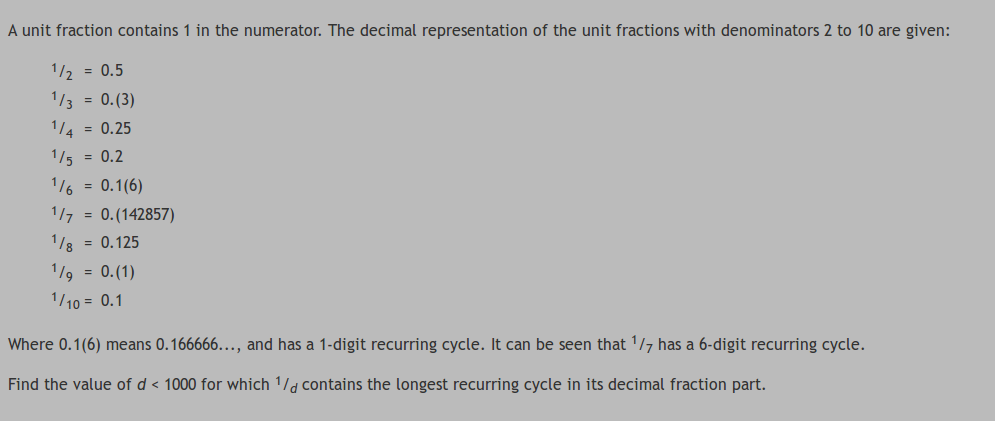
\includegraphics[scale = 0.4]{pic/026.png}
		\end{center}
	\end{figure}
\end{prob}
\begin{sol}
If $t$ is the period for number $p$, then
\begin{eqnarray}
10^{s + t} \equiv 10^s \mod p
\end{eqnarray}
If $p$ is relative prime with $2, 5$, then the above expression can be reduced to
\begin{eqnarray}
10^t \equiv 1 \mod p
\end{eqnarray}
Then brute force.
\code{code/026.py}
\end{sol}

\section{Problem 027 - Quadratic primes}
\begin{prob}
	\begin{figure}[htb!]
		\begin{center}
			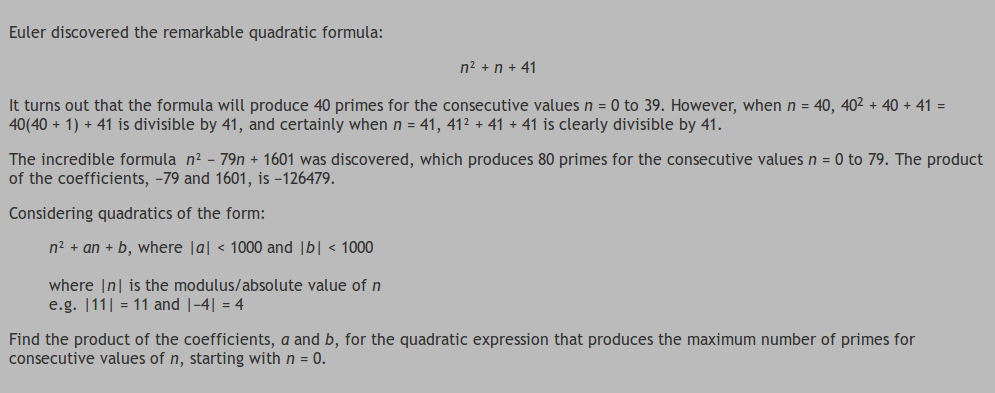
\includegraphics[scale = 0.4]{pic/027.png}
		\end{center}
	\end{figure}
\end{prob}
\begin{sol}
Brute force. But we know $b$ is a prime number between $0$ to $999$. Also we can see that when $n = b$, the result must be a compound, thus $n$ only goes from $0$ to at most $b - 1$.
\code{code/027.c}
\end{sol}

\section{Problem 028 - Number spiral diagonals}
\begin{prob}
	\begin{figure}[htb!]
		\begin{center}
			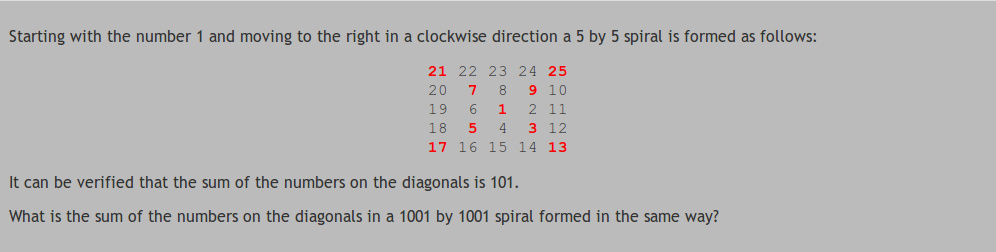
\includegraphics[scale = 0.4]{pic/028.png}
		\end{center}
	\end{figure}
\end{prob}
\begin{sol}
Deducing the formula directly may take time. We can prove that on each layer, the increment is linear to $n$, that means each layer has a sum as quadratic polynomial in $n$.
 That means the formula will take form as a cubic polynomial $f(n)$ in $n$, with $f(1) = 1, f(3) = 25, f(5) = 101, f(7) = 261$.

\begin{equation}
\begin{pmatrix}
1 & 1 & 1 & 1\\
81 & 27 & 3 & 1\\
125 & 25 & 5 & 1\\
343 & 49 & 7 & 1 
\end{pmatrix} 
\begin{pmatrix}
a\\b\\c\\d
\end{pmatrix}
 = \begin{pmatrix}
1\\25\\101\\261
\end{pmatrix}
\end{equation}
gives 
$f(n) = \dfrac{1}{6}(4 n^3 + 3n^2 + 8 n - 9)$
\end{sol}

\section{Problem 029 - Distinct powers}
\begin{prob}
	\begin{figure}[htb!]
		\begin{center}
			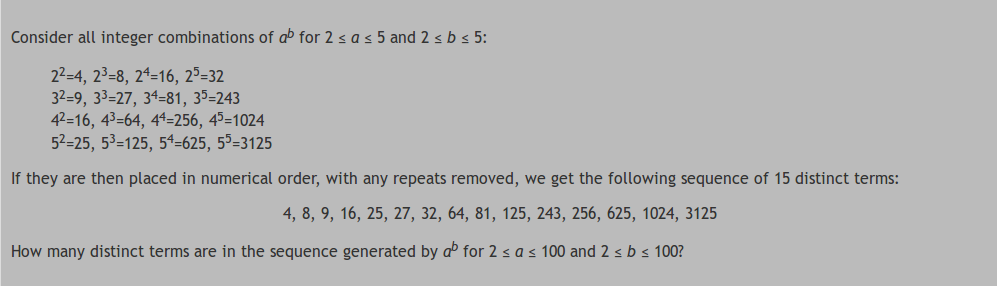
\includegraphics[scale = 0.4]{pic/029.png}
		\end{center}
	\end{figure}
\end{prob}
\begin{sol}
Brute force with \texttt{Python} one liner!
\code{code/029.py} 
\end{sol}

\section{Problem 030 - Digit fifth powers}
\begin{prob}
	\begin{figure}[htb!]
		\begin{center}
			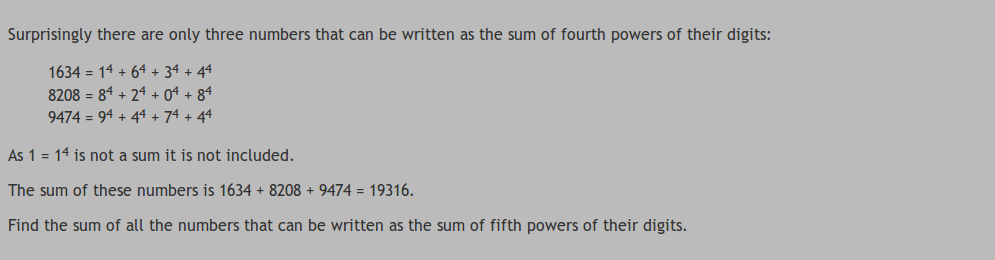
\includegraphics[scale = 0.4]{pic/030.png}
		\end{center}
	\end{figure}
\end{prob}
\begin{sol}
Brute force, since the largest number will not exceed $5 \cdot 9 ^5$.
\code{code/030.py}
\end{sol}

\section{Problem 031 - Coin sums}
\begin{prob}
	\begin{figure}[htb!]
		\begin{center}
			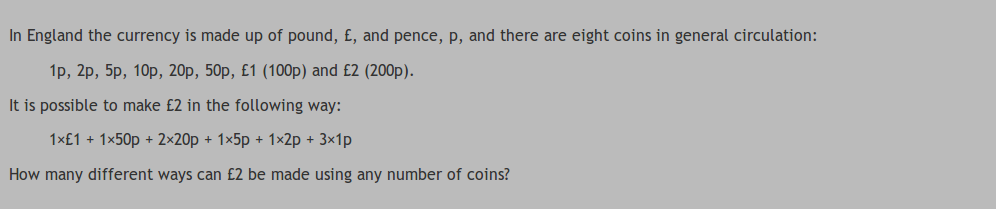
\includegraphics[scale = 0.4]{pic/031.png}
		\end{center}
	\end{figure}
\end{prob}

\begin{sol}
Consider the generating function 
$$\prod_{i}\dfrac{1}{1 - x^{n_i}}$$
We simply need to find out the coefficient of $x^{200}$. To avoid long division and observe that $n_i \mid 200$, we can use 
$$\prod_{i}\dfrac{1 - x ^ {200 + n_i}}{1 - x^{n_i}} $$
instead, that will simply require multiplication of polynomials.
\vspace{1cm}
\code{code/031.py}
\end{sol}
\section{Problem 032 - Pandigital products}
\begin{prob}
	\begin{figure}[htb!]
		\begin{center}
			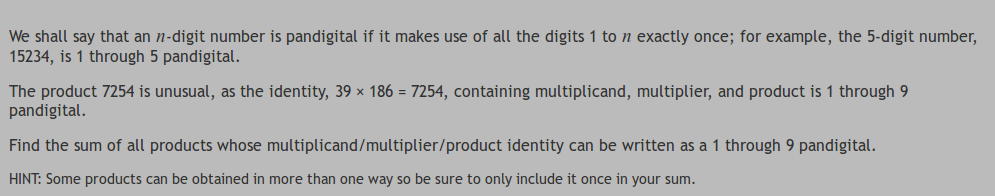
\includegraphics[scale = 0.4]{pic/032.png}
		\end{center}
	\end{figure}
\end{prob}
\begin{sol}
It is easy to show there are only two possible cases:
\begin{eqnarray}
\overline{a} \times \overline{bcde} = \overline{fghi}\\
\overline{ab}\times \overline{cde} = \overline{fghi}
\end{eqnarray}
For the first case, there are $630$ choices at most. For the second, there are $1260$ combinations.
\code{code/032.py}
\end{sol}
\newpage
\section{Problem 033}
\begin{prob}
	\begin{figure}[htb!]
		\begin{center}
			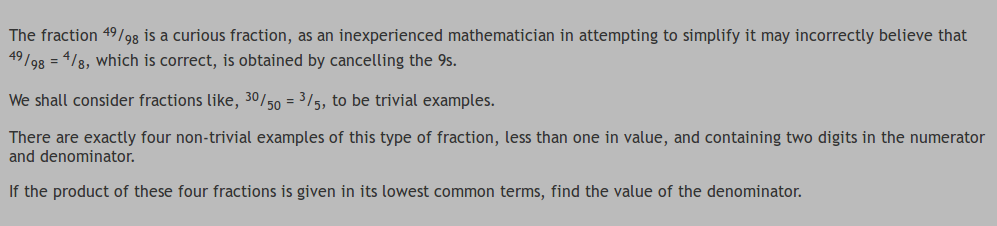
\includegraphics[scale = 0.4]{pic/033.png}
		\end{center}
	\end{figure}
\end{prob}
\section{Problem 034}
\begin{prob}
	\begin{figure}[htb!]
		\begin{center}
			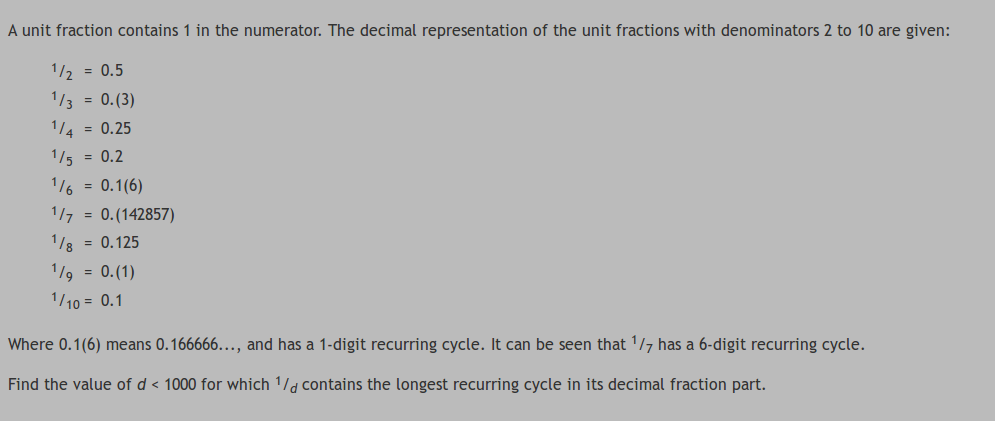
\includegraphics[scale = 0.4]{pic/026.png}
		\end{center}
	\end{figure}
\end{prob}
\section{Problem 035}
\begin{prob}
	\begin{figure}[htb!]
		\begin{center}
			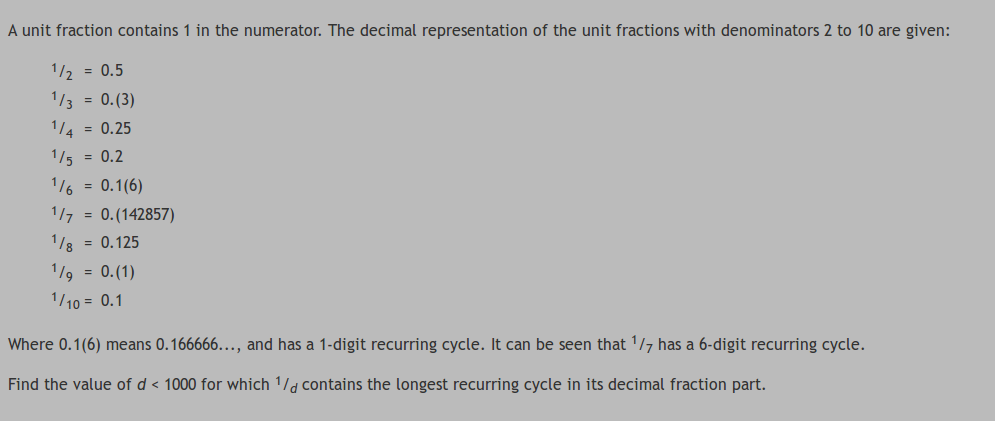
\includegraphics[scale = 0.4]{pic/026.png}
		\end{center}
	\end{figure}
\end{prob}
\section{Problem 036}
\begin{prob}
	\begin{figure}[htb!]
		\begin{center}
			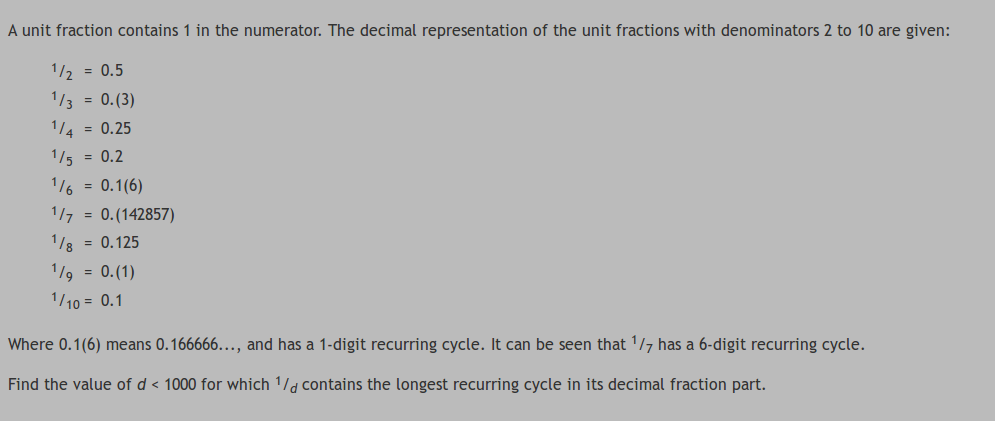
\includegraphics[scale = 0.4]{pic/026.png}
		\end{center}
	\end{figure}
\end{prob}
\section{Problem 037}
\begin{prob}
	\begin{figure}[htb!]
		\begin{center}
			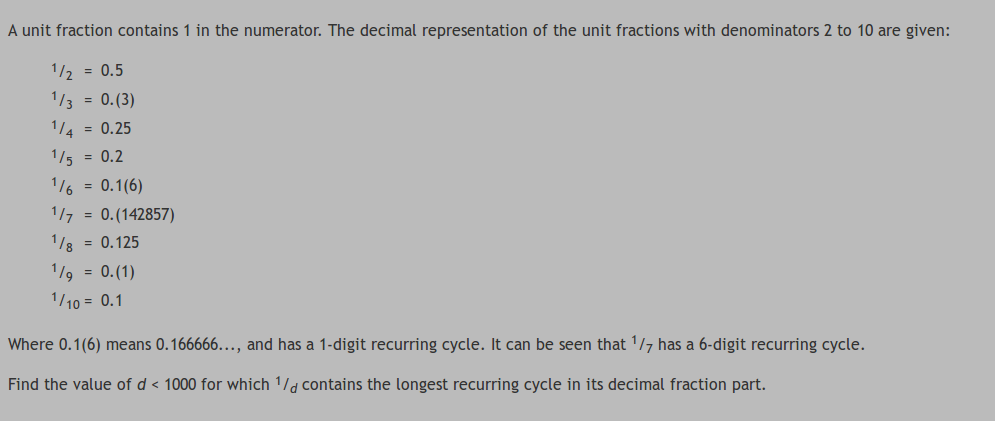
\includegraphics[scale = 0.4]{pic/026.png}
		\end{center}
	\end{figure}
\end{prob}
\section{Problem 038}
\begin{prob}
	\begin{figure}[htb!]
		\begin{center}
			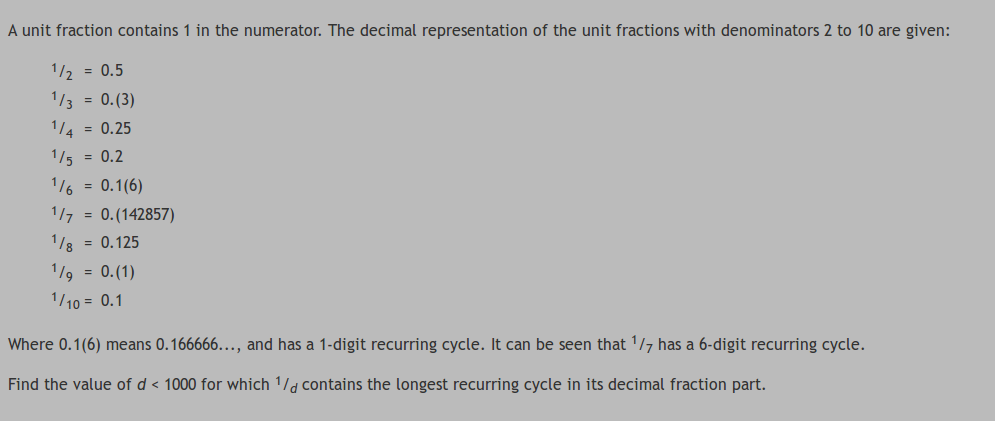
\includegraphics[scale = 0.4]{pic/026.png}
		\end{center}
	\end{figure}
\end{prob}
\section{Problem 039}
\begin{prob}
	\begin{figure}[htb!]
		\begin{center}
			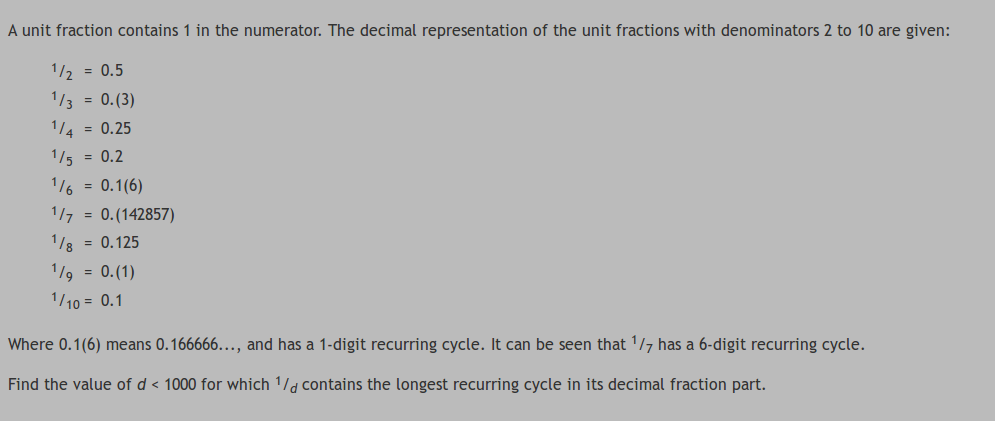
\includegraphics[scale = 0.4]{pic/026.png}
		\end{center}
	\end{figure}
\end{prob}
\section{Problem 040}
\begin{prob}
	\begin{figure}[htb!]
		\begin{center}
			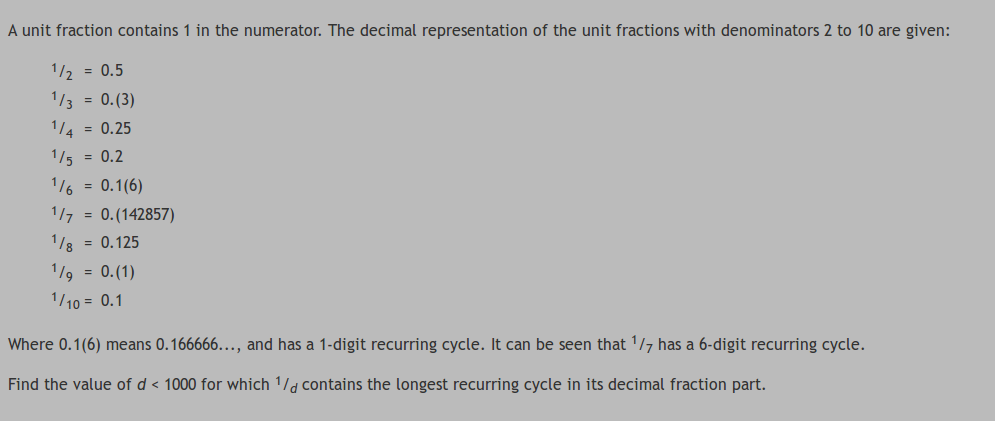
\includegraphics[scale = 0.4]{pic/026.png}
		\end{center}
	\end{figure}
\end{prob}